\chapter{Testing}

\section{Test strutturale}

\subsection{\texttt{creaOrdine()}}

\paragraph{Codice Java}

\inputminted[breaklines,tabsize=4,linenos]{java}{chapters/testing_white_box/creaOrdine.java}

\vfill

\pagebreak

\paragraph{Control Flow Graph}\mbox{}\newline

\noindent\begin{minipage}[t]{0.58\linewidth}
	\vspace{0pt}
	Il numero di cammini linearmente indipendenti è detto \emph{numero ciclomatico} di McCabe, e può essere calcolato equivalentemente in uno dei modi seguenti. Sia $G$ il grafo della funzione, allora risulta:
	\begin{enumerate}
		\item $V(G) = E - N + 2$ in cui $E = \text{\#archi in } G$, $N = \text{\#nodi in } G$
		\item $V(G) = P + 1$ con $P = \text{\#predicati in } G$
		\item $V(G) = R + 1$ con $R = \text{\#regioni chiuse in } G$
	\end{enumerate}%
	Nel nostro caso:%
	\begin{itemize}
		\item $E = 16$
		\item $N = 12$
		\item $P = 5$
		\item $R = 5$
	\end{itemize}%
	\begin{enumerate}
		\item $V(G) = E - N + 2 = 16 - 12 + 2 = 6$
		\item $P + 1 = 5 + 1 = 6$
		\item $R + 1 = 5 + 1 = 6$
	\end{enumerate}%
	\noindent I cammini di base sono:
	\begin{enumerate}
		\item 0-1
		\item 0-2
		\item 0-2-3-4-9-11
		\item 0-2-3-4-9-10-11
		\item 0-2-3-4-5-6-8-4-9-11
		\item 0-2-3-4-5-6-7-8-4-9-10-11
	\end{enumerate}
\end{minipage}
\hfill
\noindent\begin{minipage}[t]{0.38\linewidth}
	\vspace{0pt}
	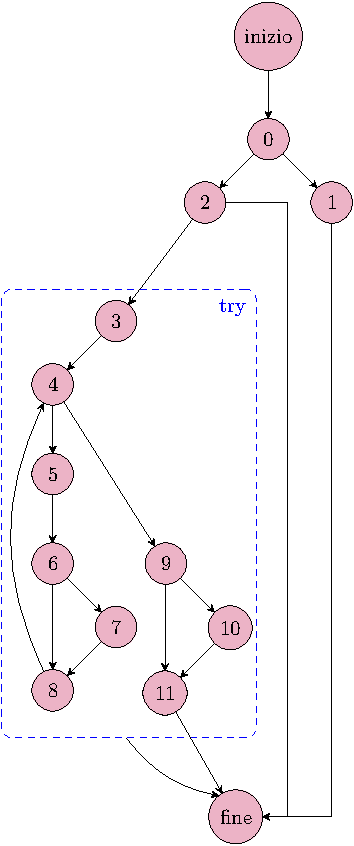
\includegraphics{chapters/testing_white_box/cfg_creaOrdine.pdf}
\end{minipage}

\vfill
\pagebreak

\paragraph{Test suite strutturale}\mbox{}\newline

\begin{table}[!hbp]
	\centering
	\begin{scenery}{colspec=lX}
		Caso d'uso: & CreaOrdine \\
		Attore primario & Cliente \\
		Attore secondario & - \\
		Descrizione & Un cliente genera un ordine contenente farmaci presenti in catalogo \\
		Pre-condizioni & Il cliente è autenticato \\
		{Sequenza di eventi \\ principale} &
			\begin{enumerate}
				\item Il cliente richiede al sistema di creare un ordine
				\item Il sistema mostra a video la lista dei farmaci
				\item Finché il cliente vuole aggiungere farmaci all'ordine
				\begin{enumerate}[label*=\arabic*.]
					\item Se viene richiesto un farmaco non da banco, il sistema chiede conferma del possesso della prescrizione
					\item Il cliente seleziona la quantità di farmaco desiderata
					\item Il sistema verifica che le scorte siano sufficienti
					\item Il sistema crea l'ordine con i farmaci inseriti e aggiorna le scorte
					\item \textit{punto di estensione}: GeneraOrdineAcquisto
				\end{enumerate}
				\item Il sistema mostra al cliente il resoconto dell'ordine e l'importo totale
				\item Se il cliente conferma l'acquisto
				\begin{enumerate}[label*=\arabic*.]
					\item Il sistema restituisce una ricevuta al cliente
				\end{enumerate}
				\item Altrimenti
				\begin{enumerate}[label*=\arabic*.]
					\item Il sistema elimina l'ordine
				\end{enumerate}
			\end{enumerate} \\
		Post-condizioni & È stato correttamente generato un ordine \\
		Casi d'uso correlati & Nessuno \\
		{Sequenza di eventi \\ alternativa} &
			\begin{enumerate}
				\item Al punto 3.1, il sistema mostra un messaggio di errore se il cliente non è in possesso della prescrizione
				\begin{enumerate}[label*=\arabic*.]
					\item Il farmaco non viene aggiunto all'ordine, il caso d'uso prosegue al punto 3
				\end{enumerate}
				\item Al punto 3.3, il sistema rileva che le scorte non sono sufficienti
					\begin{enumerate}[label*=\arabic*.]
						\item Il farmaco viene rimosso dall'ordine
					\end{enumerate}
			\end{enumerate} \\
	\end{scenery}
\end{table}


\subsection{\texttt{modificaFarmaco()}}

\paragraph{Codice Java}

\inputminted[breaklines,tabsize=4,linenos]{java}{chapters/testing_white_box/modificaFarmaco.java}

\vfill

\pagebreak

\paragraph{Control Flow Graph}\mbox{}\newline

\noindent\begin{minipage}[t]{0.58\linewidth}
	\vspace{0pt}
	Il numero di cammini linearmente indipendenti è detto \emph{numero ciclomatico} di McCabe, e può essere calcolato equivalentemente in uno dei modi seguenti. Sia $G$ il grafo della funzione, allora risulta:
	\begin{enumerate}
		\item $V(G) = E - N + 2$ in cui $E = \text{\#archi in } G$, $N = \text{\#nodi in } G$
		\item $V(G) = P + 1$ con $P = \text{\#predicati in } G$
		\item $V(G) = R + 1$ con $R = \text{\#regioni chiuse in } G$
	\end{enumerate}%
	Nel nostro caso:%
	\begin{itemize}
		\item $E = 6$
		\item $N = 5$
		\item $P = 2$
		\item $R = 2$
	\end{itemize}%
	\begin{enumerate}
		\item $V(G) = E - N + 2 = 6 - 5 + 2 = 3$
		\item $P + 1 = 2 + 1 = 3$
		\item $R + 1 = 2 + 1 = 3$
	\end{enumerate}%
	\noindent I cammini di base sono:
	\begin{enumerate}
		\item 0-1
		\item 0-1-2-4-1
		\item 0-1-2-3-4-1
	\end{enumerate}
\end{minipage}
\hfill
\noindent\begin{minipage}[t]{0.38\linewidth}
	\vspace{0pt}
	\begin{tikzpicture}[
    node/.style={circle, minimum height=20pt,text centered, draw=black, fill=purple!30},
    try/.style={rectangle, rounded corners=5, dashed, inner sep=8pt, draw=blue},
    node distance=0.8cm,
    arrow/.style={->,>=stealth}
]
\node (start) [node] {inizio};
\node (0) [node, below=of start] {$0$};
\node (1) [node, below=of 0] {$1$};
\node (2) [node, below left=of 1] {$2$};
\node (3) [node, below left=of 2] {$3$};
\node (4) [node, below=1.5cm of 2] {$4$};
\node (fine) [node, below = 4cm of 1] {fine};
\node (try) [try, fit=(0) (1) (2) (3) (4)] {};
\node [anchor=north west, inner sep=5pt, text=blue] at (try.north west) {try};



\draw[arrow] (start) -- (0);
\draw[arrow] (0) -- (1);
\draw[arrow] (1) -- (2);
\draw[arrow] (2) -- (3);
\draw[arrow] (2) -- (4);
\draw[arrow] (2) -- (4);
\draw[arrow] (3) -- (4);
\draw[arrow] (4) to [bend right=10] (1);
\draw[arrow] (1) to [bend left=50] (fine);
\draw[arrow] (try) to [bend right=10] (fine) {};

\end{tikzpicture}
\end{minipage}

\vfill
\pagebreak

\paragraph{Test suite strutturale}\mbox{}\newline

\begin{table}[!hbp]
	\centering
	\footnotesize
	\begin{tblr}{
			colspec = lXXXXX,
			hlines, vlines,
			row{1} = {font=\bfseries},
			measure=vbox
		}
		{Test \\ Case \\ ID} & Descrizione & {Cammino \\ Coperto} & Pre-condizioni & Input & Esito \\
		1 & Il farmaco è presente nel DB ma non nella collection locale, che risulta vuota & 0-1 & Il farmaco è presente nel DB ma non nella collection locale & -- &
       	Cammino non percorribile: la collection locale è sempre sincronizzata con il DB \\
		2 & La collection locale ha un solo farmaco che non è quello da modificare & 0-1-2-4-1 & -- & -- & Cammino non percorribile: se il farmaco è presente nel DB, deve essere presente anche nella collection locale \\
		3 & Il farmaco esiste & 0-1-2-3-4-1 & Il farmaco esiste & {Nome: Plasil \\ Prezzo: 11.50 \euro \\ Scorte: 30 \\ Prescrizione: \texttt{True}} & Farmaco modificato \\
	\end{tblr}
\end{table}
